\documentclass[12pt,a4paper,]{report}

% ams
\usepackage{amssymb,amsmath}

\usepackage{ifxetex,ifluatex}
\usepackage{fixltx2e} % provides \textsubscript
\ifnum 0\ifxetex 1\fi\ifluatex 1\fi=0 % if pdftex
  \usepackage[T1]{fontenc}
  \usepackage[utf8]{inputenc}
\else % if luatex or xelatex
  \makeatletter
  \@ifpackageloaded{fontspec}{}{\usepackage{fontspec}}
  \makeatother
  \defaultfontfeatures{Ligatures=TeX,Scale=MatchLowercase}
  \makeatletter
  \@ifpackageloaded{soul}{
     \renewcommand\allcapsspacing[1]{{\addfontfeature{LetterSpace=15}#1}}
     \renewcommand\smallcapsspacing[1]{{\addfontfeature{LetterSpace=10}#1}}
   }{}
  \makeatother

% hard-coded fonts
\setmainfont[]{Roboto}
\setmonofont[]{Roboto}

\fi



% geometry
\usepackage[includehead, hmargin={3cm,3cm}, vmargin={2cm,3cm}, headsep=1.2cm, footskip=1.2cm]{geometry}

% figures placement
\usepackage{floatrow}
\floatsetup[figure]{capposition=top}
\floatplacement{figure}{H}

% headers
\usepackage{fancyhdr}
\renewcommand{\headruleskip}{10pt} %distance between headrule and header content
\renewcommand{\footnoterule}{\vfill\kern -3pt \hrule width 0.4\columnwidth \kern 2.6pt}

\pagestyle{fancy}
\fancyhead[R]{
\includegraphics[height=15pt]{logos/schola}}

\fancyhead[L]{
\includegraphics[height=25pt]{logos/eduzmena}}
\setlength{\headheight}{25pt}


% atypical captions above figures
\usepackage{caption}
\captionsetup{justification=raggedright,singlelinecheck=false,belowskip=0pt}

% graphix
\usepackage{graphicx}
\setkeys{Gin}{width=\linewidth,totalheight=\textheight,keepaspectratio}

% booktabs
\usepackage{booktabs}

% url
\usepackage{url}

% hyperref
\usepackage{hyperref}

% units.
\usepackage{units}

% use babel whatever engine is used
  \usepackage[shorthands=off,main=czech]{babel}

\addto\captionsenglish{\renewcommand{\figurename}{Fig.}}
\addto\captionsczech{\renewcommand{\figurename}{Graf}}

% microtype for better kernign etc.
\RequirePackage[final,babel=true]{microtype}
\DeclareMicrotypeBabelHook
  {czech}
  {kerning=, spacing=}

\setcounter{secnumdepth}{-1} %??

% citations


% pandoc syntax highlighting

% longtable
\usepackage{longtable,booktabs}

% multiplecol
\usepackage{multicol}

% strikeout
\usepackage[normalem]{ulem}

% morefloats
\usepackage{morefloats}

% spacing
\usepackage{setspace}

\newcommand{\tr}[2]{\ifnum\pdfstrcmp{\languagename}{czech}=0 #1\else #2\fi}

% tightlist macro required by pandoc >= 1.14
\providecommand{\tightlist}{%
  \setlength{\itemsep}{0pt}\setlength{\parskip}{0pt}}


\begin{document}

\begin{titlepage}
    \begin{center}

      \onehalfspacing

      \vspace*{1cm}

      \begin{figure}
      \centering
      
\includegraphics[width=4cm]{logos/eduzmena}%
      \hspace{1.5cm}%
      
\includegraphics[width=6.5cm]{logos/schola}%
      \end{figure}

      \vspace{1cm}

      \textbf{\huge Výsledky z dotazníku pro učitele}

      \vspace{.25cm}

      \textit{\Large Základní škola Zvoleněves, okres Kladno\\
RED IZO: 600044467}

      \vspace{1cm}

      \large

      1. března 2021

      \vspace{1cm}

      výzkumný tým SCHOLA EMPIRICA

      \vspace{.25cm}

            Magdaléna Klimešová\footnote{Korespondenční autor. Kontakt: \href{mailto:klimesova@scholaempirica.org}{\nolinkurl{klimesova@scholaempirica.org}}}, Jaromír Mazák, Jan Netík, Aleš Vomáčka, Martina Koutná \tr{a}{and} Marek Havrda

      \vspace{1.5cm}

    \end{center}
\end{titlepage}


\thispagestyle{empty}
\section*{Shrnutí}
Zpráva seznamuje čtenáře s výsledky šetření mezi učiteli v rámci projektu Eduzměna, u kterých jsme mapovali situaci v celé řadě oblastí. Šlo zejména o vnímání školního prostředí, sebehodnocení pedagogických dovedností a víru v dopady své práce, otázky seberozvoje, mentoringu a účinku zpětné vazby, vnímané autonomie a podpory ze strany vedení školy, komunikaci a spolupráci s různými aktéry, spokojenost s prací a potenciální pracovní stresory, vnímání odměny, prestiže pedagogické profese a školy jako celku. Zmíněné oblasti jsme mapovali pomocí online dotazníku, jehož sběr probíhal v rozmezí 9.--26. října 2020.


{
\renewcommand*\contentsname{Obsah zprávy}
\setcounter{tocdepth}{1}
\tableofcontents
}

\newpage

\hypertarget{jak-se-zpruxe1vou-pracovat}{%
\chapter{Jak se zprávou pracovat}\label{jak-se-zpruxe1vou-pracovat}}

Jednotlivé položky dotazníku, z nichž velká část vychází z ověřených mezinárodních šetření typu TALIS či PISA, jsou sdružovány do tzv. škál (dimenzí) postihujících určité koncepty nebo oblasti. Položky se ptají na postoje respondentů, na to, jak danou otázku vnímají. Škály, které uvidíte na následujících stranách, ukazují vždy průměr z příslušných položek\footnote{Jednotlivým kategoriím odpovědí se přiřazují přirozená, po sobě jsoucí čísla. Např. „rozhodně nesouhlasím -- rozhodně souhlasím`` se očíslují 1--4, a číslo tak vyjadřuje míru souhlasu.} (konkrétní znění je k vidění v příloze). Škály prezentujeme tak, že žádoucí je vždy vyšší bodový zisk (a to i u škály „Pracovní vytížení a stres``, jejíž původní bodování je pro jednotnost v tomto dotazníku „otočeno``). Podle mediánu\footnote{Pokud bychom seřadili výsledky jednotlivých učitelů podle počtu bodů v dotazníku či vybraném souboru otázek, pak medián označuje hodnotu \emph{právě uprostřed} takové řady. Pokud je učitelů sudý počet, jde o průměr prostřední dvojice učitelů.} získaných bodů také jednotlivé škály řadíme. Vizualizace všech položek dotazníku, které tvoří jednotlivé škály, jsou prezentovány v příloze.

Zpráva je sestavena s cílem poskytnout rychlý vhled. Tematické sekce, podle kterých byl dotazník členěn, jsou zde částečně potlačeny a snažíme se maximum informací prezentovat pokud možno v kompaktní grafické podobě. Ve zprávě využíváme dva typy grafů:

\begin{itemize}
\tightlist
\item
  \textbf{krabicový graf} (angl. \emph{boxplot}), který přehledně zobrazuje typické hodnoty -- silnější linka vyznačuje medián, šedá, vyplněná část ohraničuje 50 \% prostředních hodnot kolem mediánu (tj. mezi 25. a 75. percentilem, na obrázku jako IQR), horizontální úsečky pak poukazují na 1,5násobek tohoto rozpětí. Hodnoty mimo představují mimořádně odlehlá pozorování či extrémy (tvoří dohromady méně než 1 \% dat). Samotné hodnoty jsou na ose „x`` (horizontální osa) a tato osa má vždy rozsah podle toho, kolik bodů je možné získat.
\end{itemize}

\begin{figure}
\centering
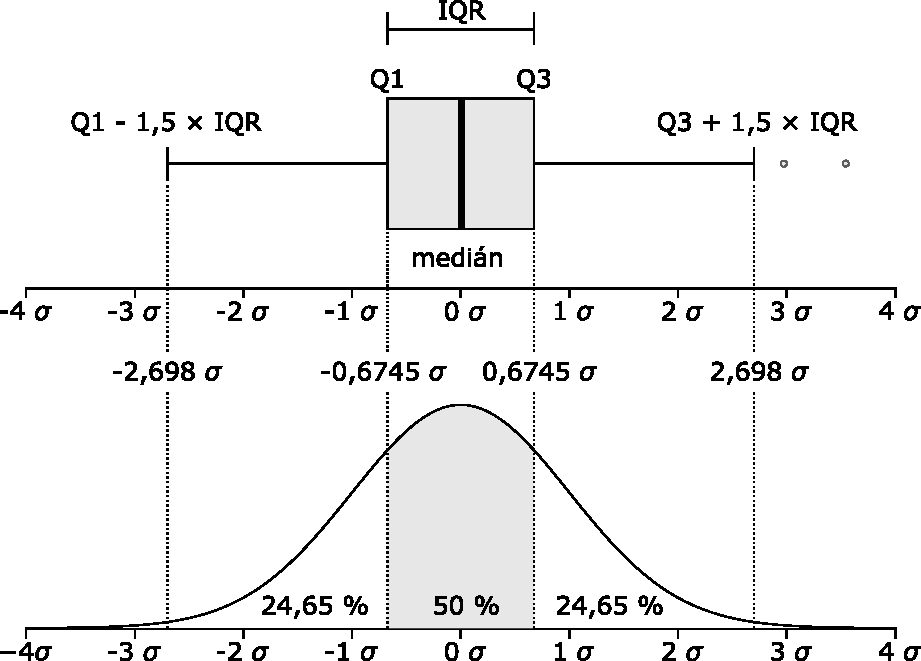
\includegraphics{figures/boxplot_description.pdf}
\caption{Obr. 1. Popis krabicového grafu (\(\sigma\) značí směrodatnou odchylku, spodní část obrázku znázorňuje rozložení hodnot)}
\end{figure}

\begin{itemize}
\tightlist
\item
  \textbf{skládaný sloupcový graf} (angl. \emph{stacked barplot}) vizualizuje podíl jednotlivých odpovědí pro jednotlivé položky dotazníku. Osa „x`` je tedy vyjádřená v procentech.
\end{itemize}

\hypertarget{vuxfdsledky}{%
\chapter{Výsledky}\label{vuxfdsledky}}

Níže prezentujeme výsledky odpovědí na otázky pro všechny škály s rozsahem 1--4 body s tím, že žádoucí je vždy vyšší bodový zisk.

\begin{figure}

{\centering 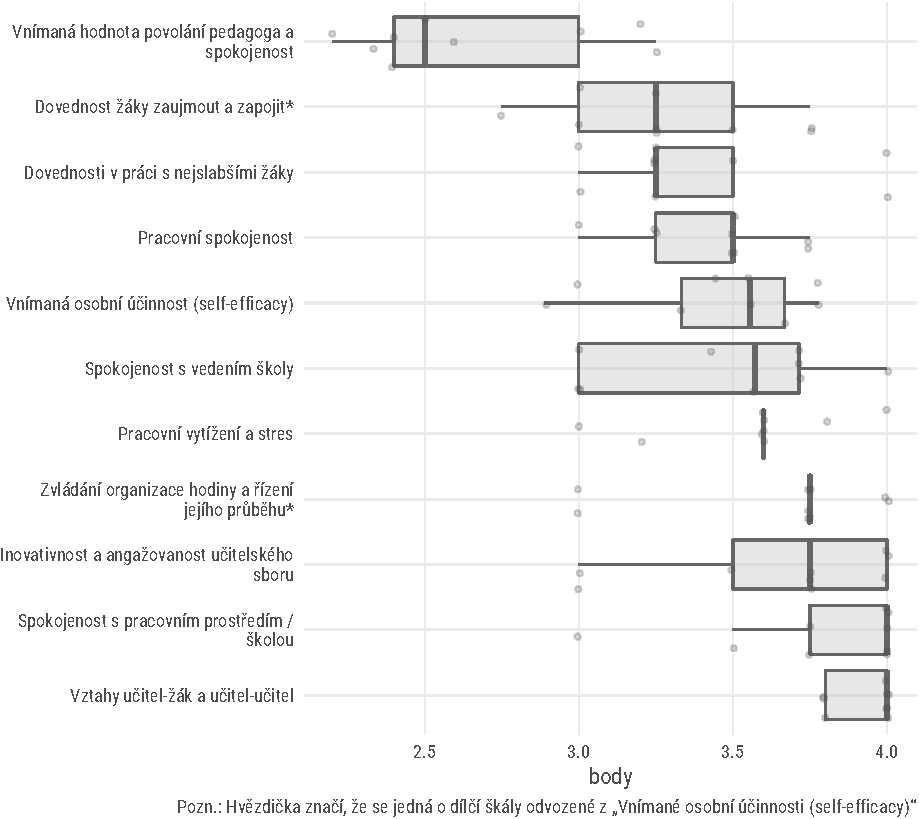
\includegraphics[width=\textwidth]{figs/scales1to4-1}

}

\caption{Všechny škály s rozsahem 1--4 body}\label{fig:scales1to4}
\end{figure}

\begin{figure}

{\centering 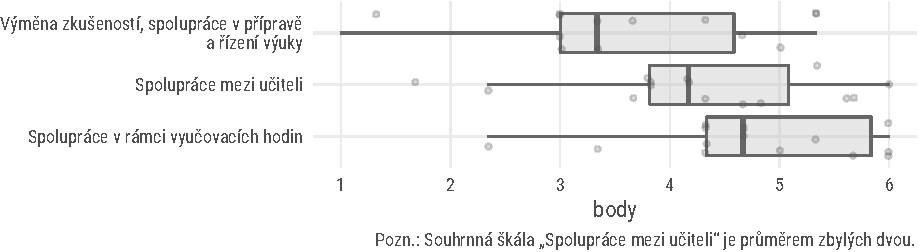
\includegraphics[width=\textwidth]{figs/scales1to6-1}

}

\caption{Spolupráce mezi učiteli (škály s rozsahem 1--6 bodů)}\label{fig:scales1to6}
\end{figure}

\newpage

Následující grafy ukazují položky, které nenáleží do žádné škály, a tak je prezentujeme samostatně. Dělení do skupin vychází čistě z možností odpovědí (otázky mají stejnou legendu). Pro lepší orientaci řadíme položky podle součtu dvou nejvíce kladných možností.

\begin{figure}

{\centering 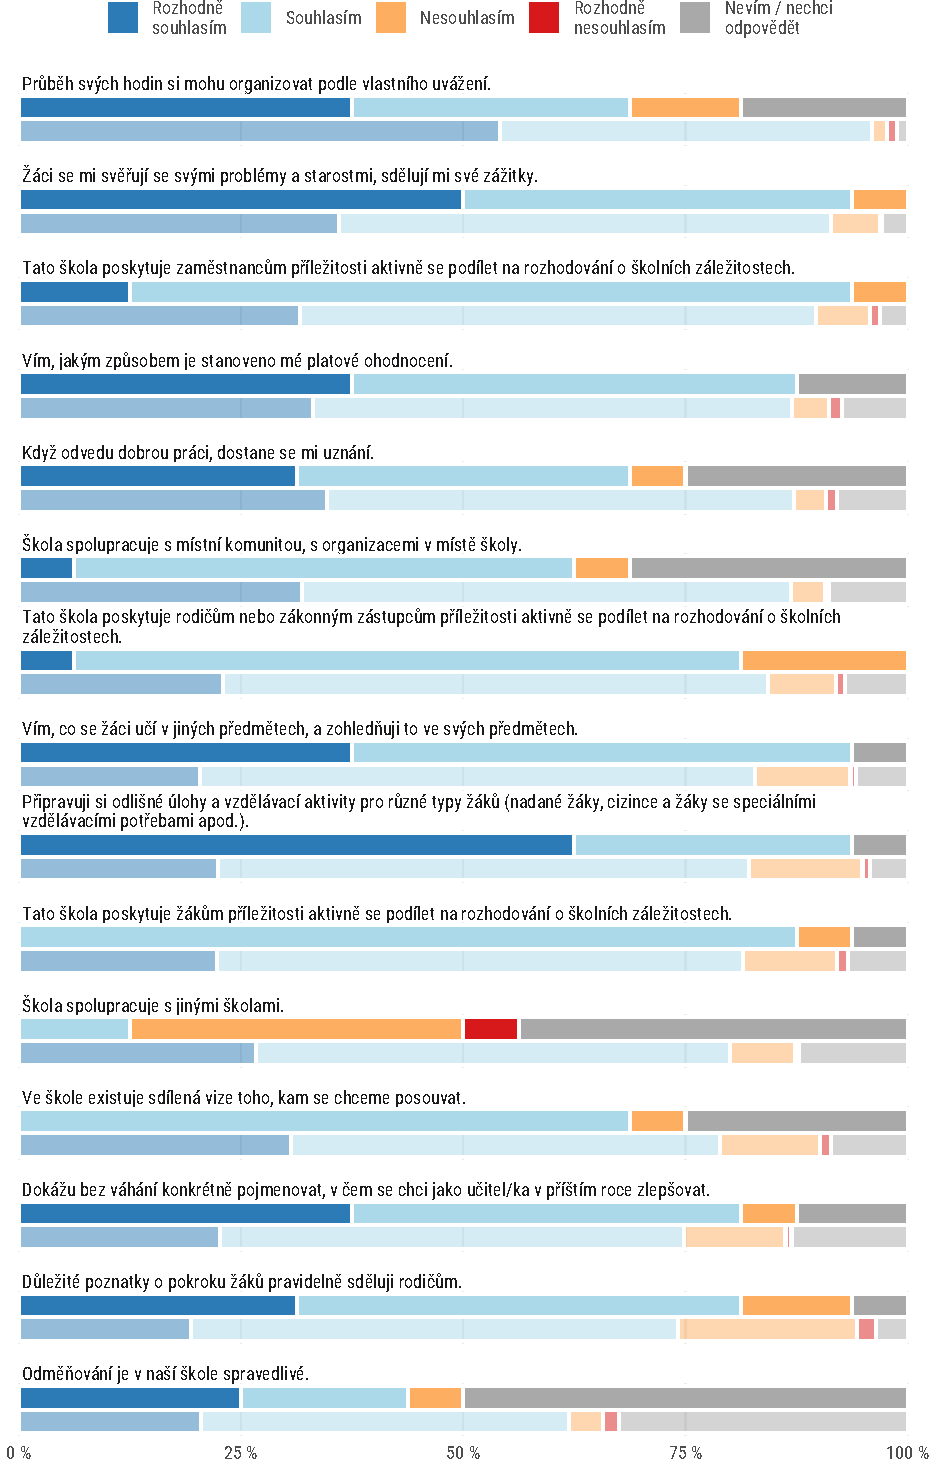
\includegraphics[width=\textwidth]{figs/likert-1}

}

\caption{Položky vyjadřující míru souhlasu pomocí 4 kategorií}\label{fig:likert}
\end{figure}

\begin{figure}

{\centering 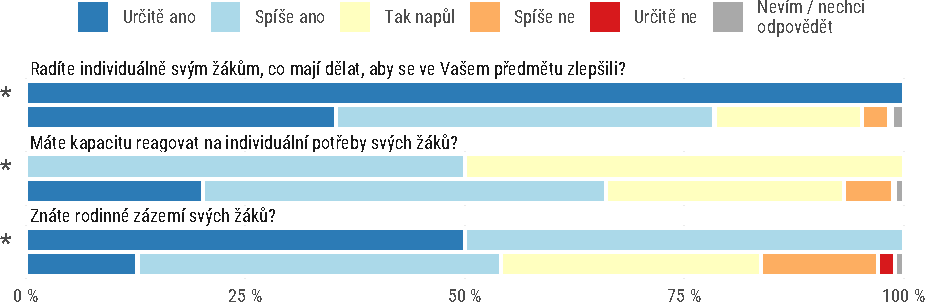
\includegraphics[width=\textwidth]{figs/midpoint-1}

}

\caption{Položky vyjadřující míru souhlasu pomocí 5 kategorií}\label{fig:midpoint}
\end{figure}

\begin{figure}

{\centering 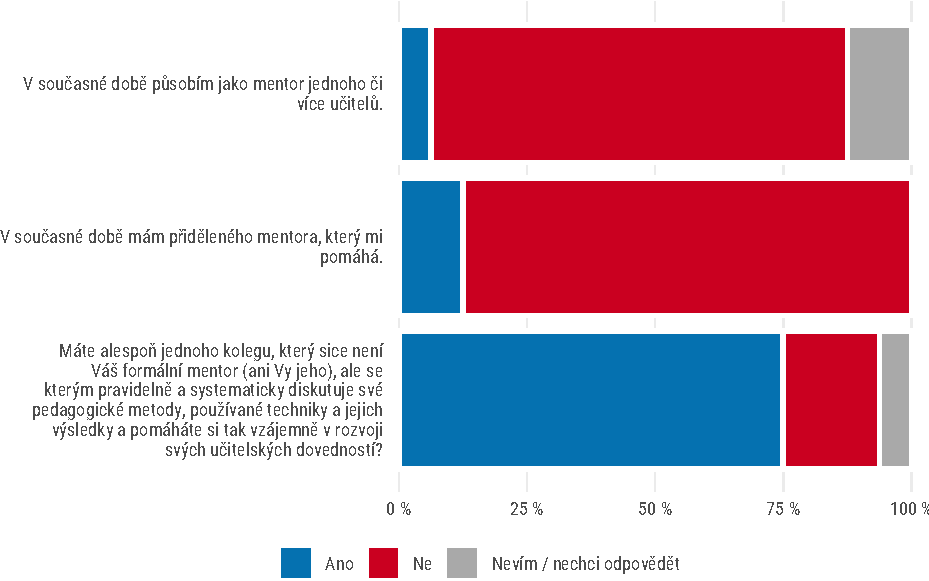
\includegraphics[width=\textwidth]{figs/mentoring-1}

}

\caption{Formální i neformální mentorství}\label{fig:mentoring}
\end{figure}

\begin{figure}

{\centering 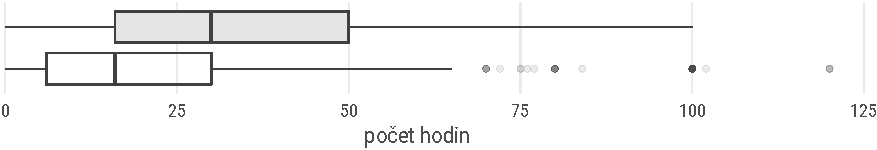
\includegraphics[width=\textwidth]{figs/profDevelop-1}

}

\caption{Účast na přednáškách, workshopech či jiných odborných akcích věnovaných profesnímu rozvoji z vlastního zájmu (nad rámec povinného vzdělávání) za minulé pololetí}\label{fig:profDevelop}
\end{figure}

\newpage

Následující graf (č. \ref{fig:feedback}) vizualizuje odpovědi 13 učitelů (81 \%), kteří vnímají pozitivní dopad obdržené zpětné vazby na styl své výuky. Opak uvedli pouze 2 učitelé (12 \%).

\begin{figure}

{\centering 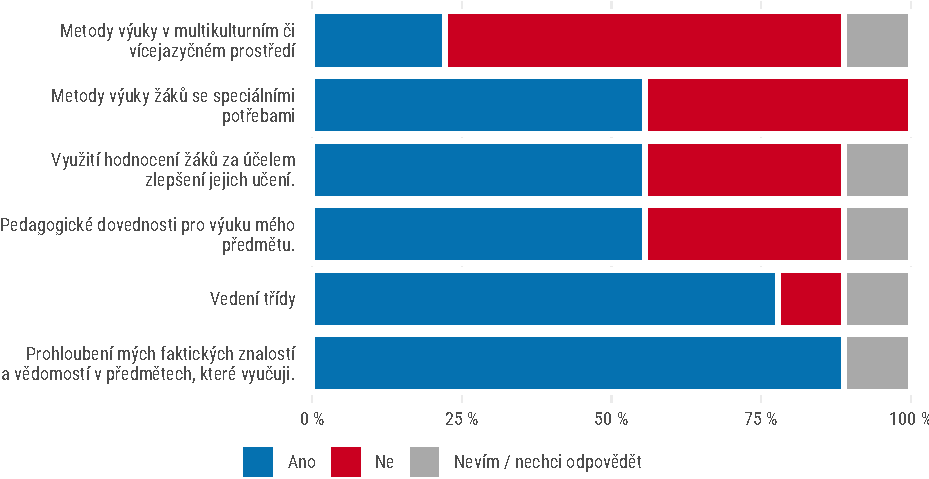
\includegraphics[width=\textwidth]{figs/feedback-1}

}

\caption{Vnímání pozitivního dopadu zpětné vazby na jednotlivé aspekty výuky}\label{fig:feedback}
\end{figure}

\hypertarget{zuxe1kladnuxed-uxfadaje-o-respondentech}{%
\chapter{Základní údaje o respondentech}\label{zuxe1kladnuxed-uxfadaje-o-respondentech}}

Tato sekce shrnuje základní, zejména sociodemografické údaje o učitelích, kteří dotazník vyplnili. Dále zachycuje jejich pedagogické zkušenosti, délku učitelského úvazku a zprostředkovaně také motivaci k volbě povolání (viz graf č. \ref{fig:career}). Graf č. \ref{fig:subjects} odkazuje na skladbu vyučovaných předmětů, resp. jejich kategorií.

Celkem 24 učitelů dotazník otevřelo a 16 ho vyplněný odeslalo. Efektivní návratnost je tedy 67 \%.

Běžný počet přeskočených nepovinných položek je 3, „únikových`` voleb typu „Nevím / nechci odpovědět`` pak učitelé běžně využívali 3,5krát. 2 učitel/é tuto možnost volil/i mimořádně často -- nejvíce 28krát.

\begin{figure}

{\centering 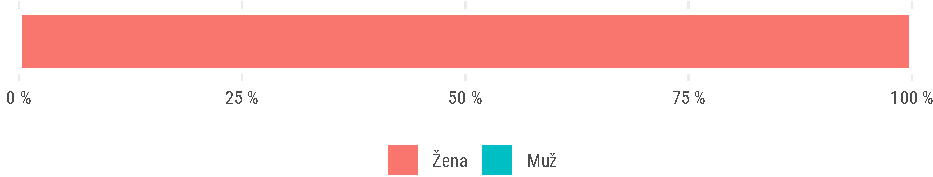
\includegraphics[width=\textwidth]{figs/sex-1}

}

\caption{Zastoupení pohlaví}\label{fig:sex}
\end{figure}

\begin{figure}

{\centering 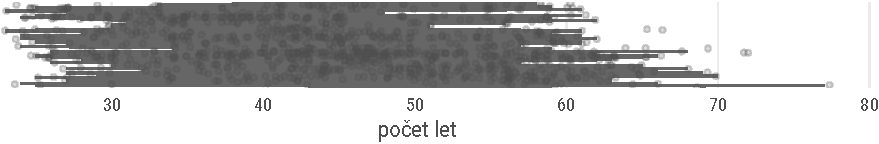
\includegraphics[width=\textwidth]{figs/age-1}

}

\caption{Věk}\label{fig:age}
\end{figure}

\begin{figure}

{\centering 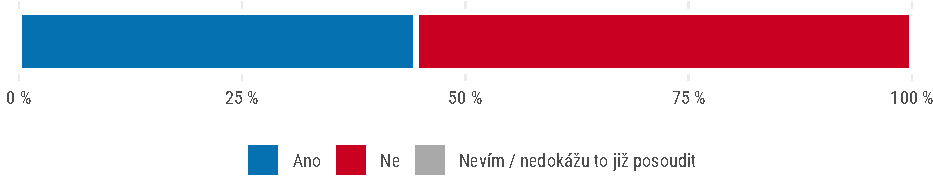
\includegraphics[width=\textwidth]{figs/career-1}

}

\caption{Učitelská profese jako první kariérní volba}\label{fig:career}
\end{figure}

\begin{figure}

{\centering 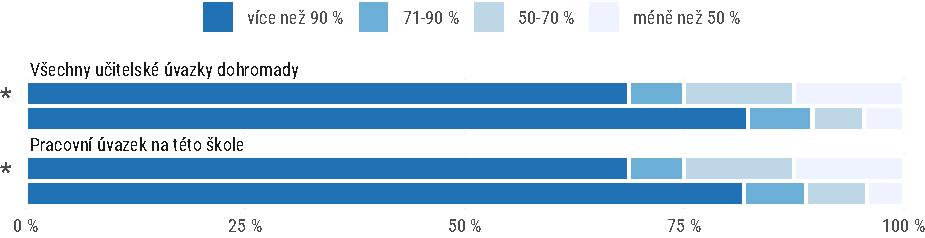
\includegraphics[width=\textwidth]{figs/job-1}

}

\caption{Současné pracovní úvazky na pozici učitele}\label{fig:job}
\end{figure}

\begin{figure}

{\centering 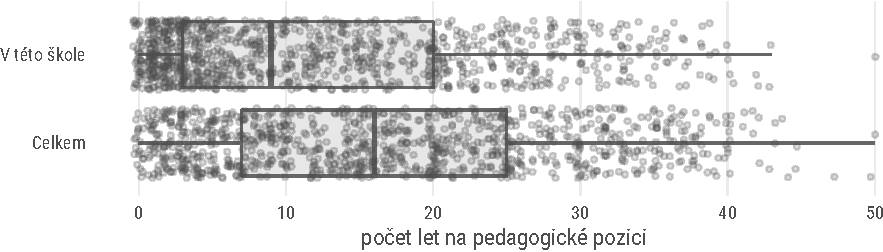
\includegraphics[width=\textwidth]{figs/yearsTeach-1}

}

\caption{Pracovní zkušenosti}\label{fig:yearsTeach}
\end{figure}

Celkem 1 (tj. cca 6 \%) učitelů nebo učitelek vyučuje výhradně na 2. stupni. Následující graf tedy ukazuje procento výuky na 1. stupni reportované \emph{zbývajícími učiteli}. Bod na úrovni 75~\% znamená, že daný učitel vyučuje 75~\% času na prvním stupni a 25~\% na stupni druhém.

\begin{figure}

{\centering 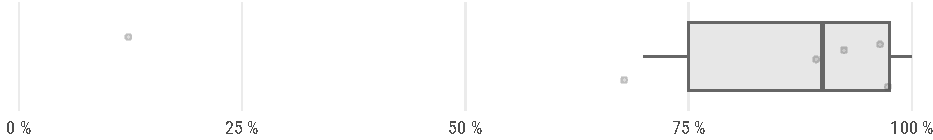
\includegraphics[width=\textwidth]{figs/s8q2-1}

}

\caption{Podíl výuky na prvním stupni}\label{fig:s8q2}
\end{figure}

\begin{figure}

{\centering 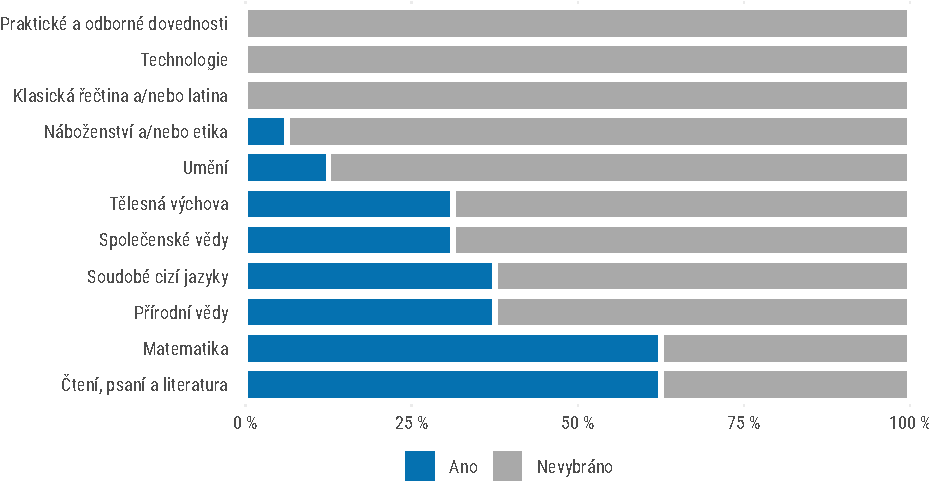
\includegraphics[width=\textwidth]{figs/subjects-1}

}

\caption{Počty pedagogů vyučujících jednotlivé kategorie předmětů}\label{fig:subjects}
\end{figure}

Učitelé mají na starosti výuku různých předmětů, které vyobrazujeme v 11 kategoriích, jak je běžné v mezinárodních šetření typu PISA či TALIS. Modrá výplň ukazuje počet učitelů, kteří předmět či kategorii vyučují nebo vyučovali v tomto nebo předchozím školním roce. Platí, že jeden učitel může vyučovat více předmětů.

\newpage

\hypertarget{pux159uxedloha}{%
\chapter{Příloha}\label{pux159uxedloha}}

\hypertarget{vizualizace-poloux17eek-dotaznuxedku-tvoux159uxedcuxedch-ux161kuxe1ly}{%
\section{Vizualizace položek dotazníku tvořících škály}\label{vizualizace-poloux17eek-dotaznuxedku-tvoux159uxedcuxedch-ux161kuxe1ly}}

Škály, které jste viděli na začátku zprávy, sestávají vždy z několika položek, na které se odpovídá stejným způsobem (např. míra souhlasu). V následující příloze si můžete podrobně prohlédnout, z jakých konkrétních otázek daná škála vychází a jak na ní učitelky a učitelé ve vaší škole odpovídali.

\begin{figure}

{\centering 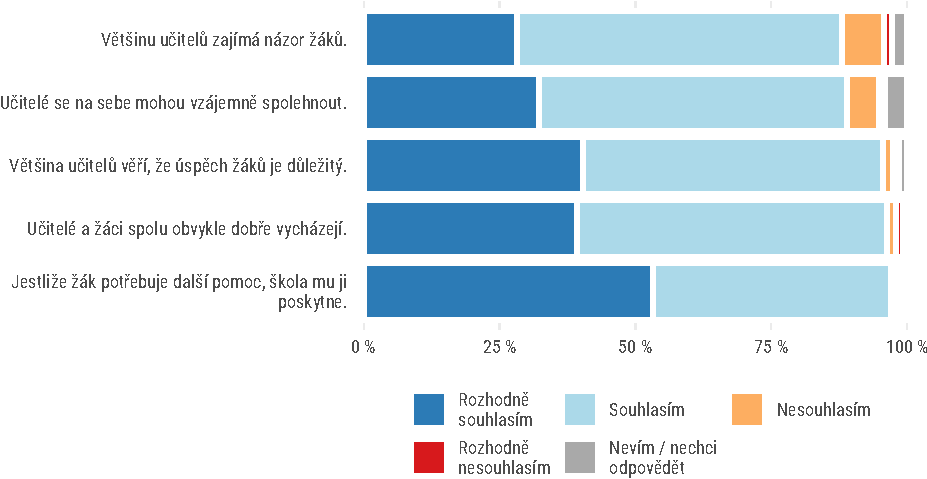
\includegraphics[width=\textwidth]{figs/tots1q1T3STUDappdx-1}

}

\caption{Vztahy učitel-žák a učitel-učitel}\label{fig:tots1q1T3STUDappdx}
\end{figure}

\begin{figure}

{\centering 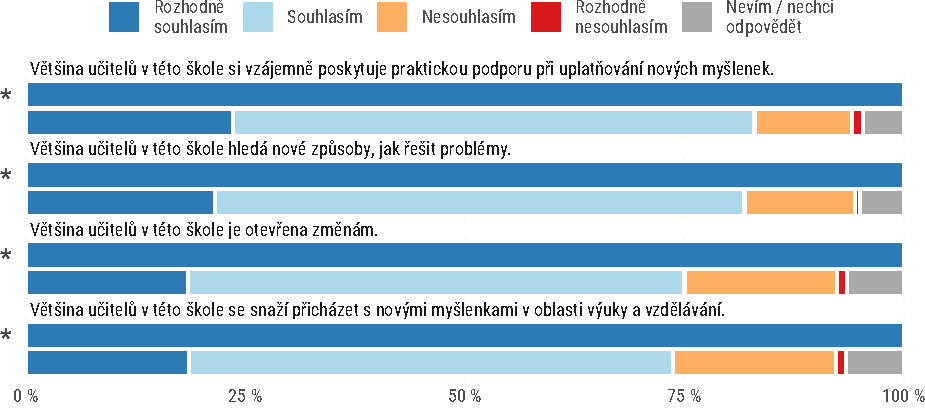
\includegraphics[width=\textwidth]{figs/tots1q3T3TEAMappdx-1}

}

\caption{Inovativnost a angažovanost učitelského sboru}\label{fig:tots1q3T3TEAMappdx}
\end{figure}

\begin{figure}

{\centering 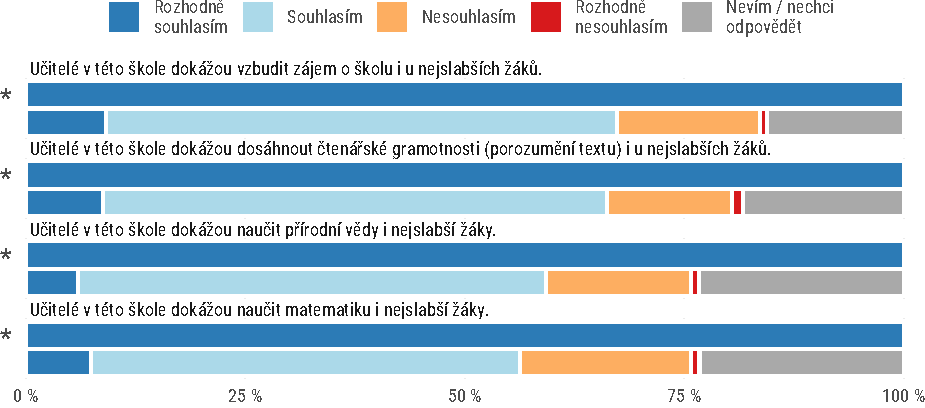
\includegraphics[width=\textwidth]{figs/tots1q4weakappdx-1}

}

\caption{Dovednosti v práci s nejslabšími žáky}\label{fig:tots1q4weakappdx}
\end{figure}

\begin{figure}

{\centering 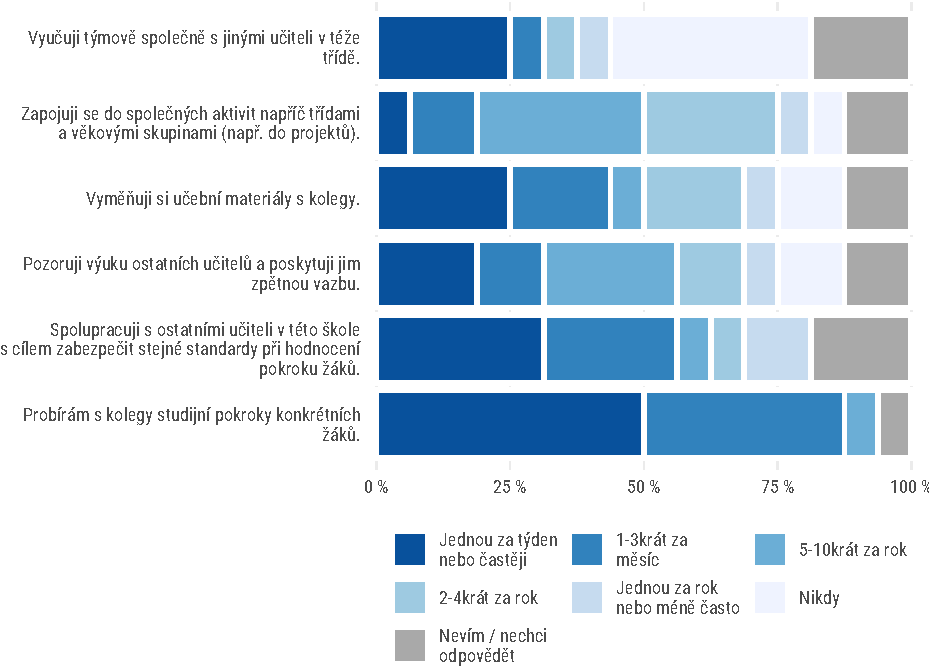
\includegraphics[width=\textwidth]{figs/tots2q1T3COOPappdx-1}

}

\caption{Spolupráce mezi učiteli}\label{fig:tots2q1T3COOPappdx}
\end{figure}

\begin{figure}

{\centering 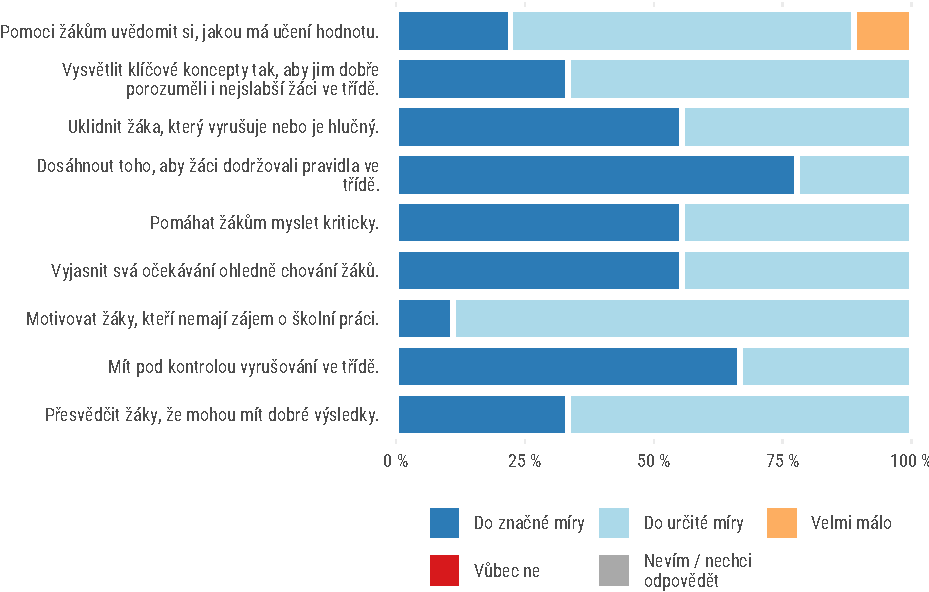
\includegraphics[width=\textwidth]{figs/tots2q2T3SELFappdx-1}

}

\caption{Vnímaná osobní účinnost (self-efficacy)}\label{fig:tots2q2T3SELFappdx}
\end{figure}

\begin{figure}

{\centering 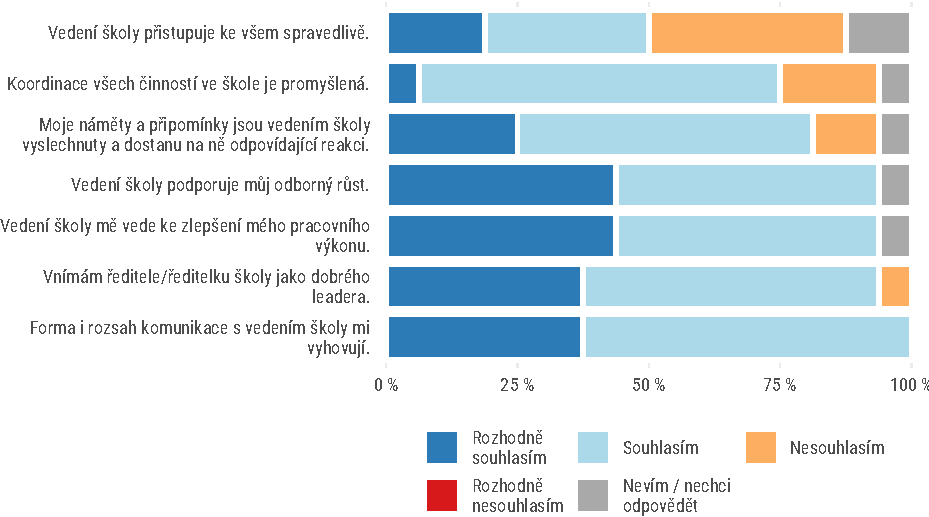
\includegraphics[width=\textwidth]{figs/tots4q3leaderappdx-1}

}

\caption{Spokojenost s vedením školy}\label{fig:tots4q3leaderappdx}
\end{figure}

\begin{figure}

{\centering 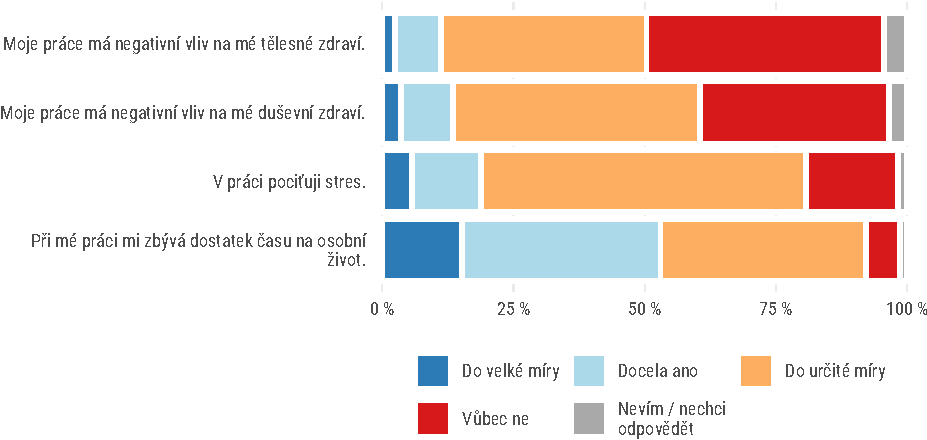
\includegraphics[width=\textwidth]{figs/tots6q1T3WELSappdx-1}

}

\caption{Pracovní spokojenost}\label{fig:tots6q1T3WELSappdx}
\end{figure}

\begin{figure}

{\centering 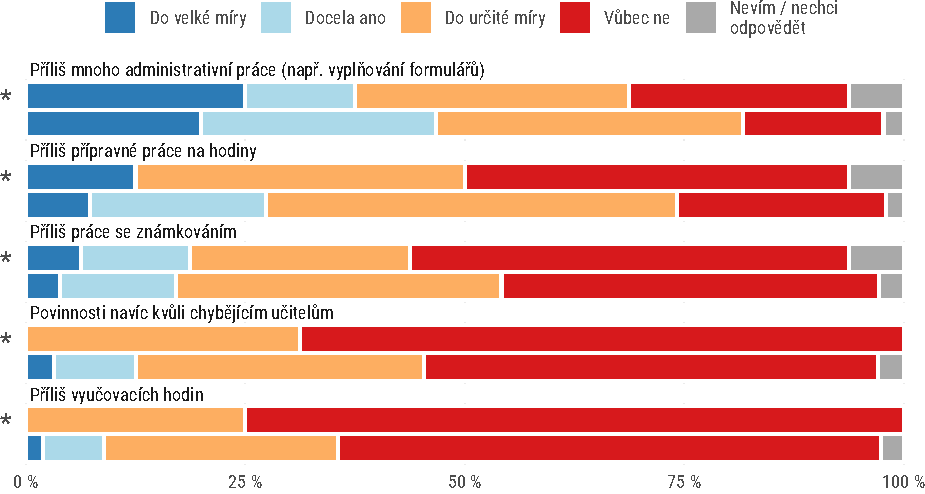
\includegraphics[width=\textwidth]{figs/tots6q2T3WLOADappdx-1}

}

\caption{Pracovní vytížení a stres}\label{fig:tots6q2T3WLOADappdx}
\end{figure}

\begin{figure}

{\centering 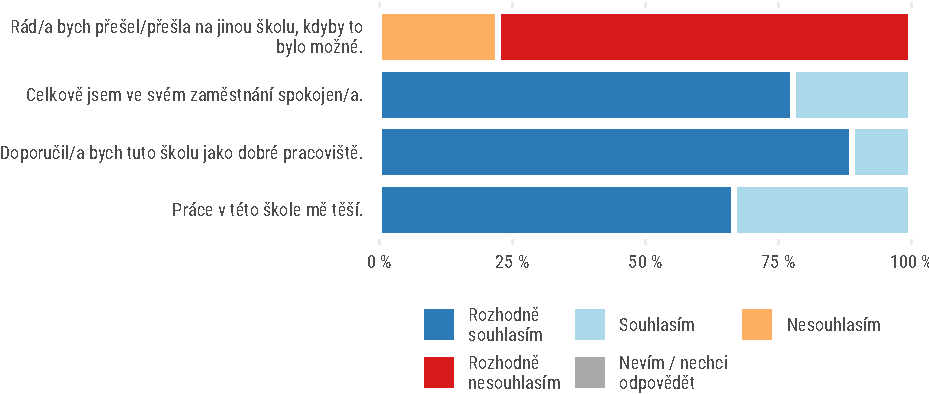
\includegraphics[width=\textwidth]{figs/tots6q4T3JSENVappdx-1}

}

\caption{Spokojenost s pracovním prostředím / školou}\label{fig:tots6q4T3JSENVappdx}
\end{figure}

\begin{figure}

{\centering 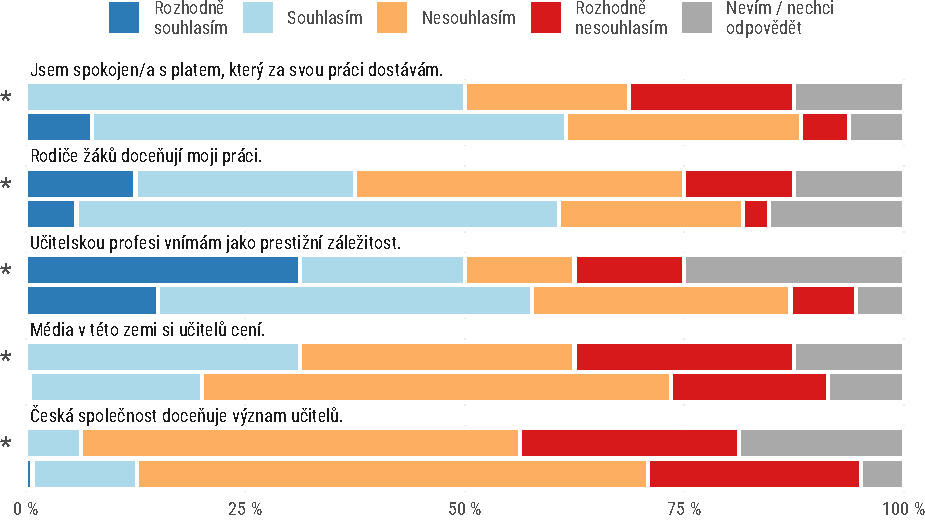
\includegraphics[width=\textwidth]{figs/tots7q1teachperceptappdx-1}

}

\caption{Vnímaná hodnota povolání pedagoga a spokojenost}\label{fig:tots7q1teachperceptappdx}
\end{figure}



\end{document}
